\documentclass[11pt]{article}
\usepackage[utf8]{inputenc}
\usepackage{polski} 
\usepackage{geometry}
\geometry{a4paper}
\usepackage{graphicx}
\usepackage{booktabs}
\usepackage{array}
\usepackage{paralist}
\usepackage{verbatim}
\usepackage{subfig}
\usepackage{amsmath}
\usepackage{float}
\usepackage{amsthm}
\usepackage{amssymb}
\usepackage{amsfonts}
\usepackage{thmtools}
\theoremstyle{definition}
\newtheorem{zad}{Zadanie}
\numberwithin{zad}{section}

\newtheorem{theorem}{Twierdzenie}
\newtheorem{definition}{Definicja}
\newtheorem{lemma}{Lemat}
\renewcommand*{\proofname}{Rozwiązanie}

\usepackage{fancyhdr}
\pagestyle{fancy}
\renewcommand{\headrulewidth}{0pt}
\usepackage{sectsty}
\usepackage{float}
\allsectionsfont{\sffamily\mdseries\upshape}
\usepackage[nottoc,notlof,notlot]{tocbibind}
\usepackage[titles,subfigure]{tocloft}
\renewcommand{\cftsecfont}{\rmfamily\mdseries\upshape}
\renewcommand{\cftsecpagefont}{\rmfamily\mdseries\upshape}

\title{Matematyka}

\begin{document}
\maketitle
\tableofcontents


\section{Zadania}
\subsection{Zabawy z liczbami}

\begin{zad}
Rok wydania dzieła Kopernika \textit{O obrotach ciał niebieskich} jest liczbą czterocyfrową, której suma cyfr wynosi 13, cyfra dziesiątek stanowi $80\%$ cyfry setek, a cyfra tysięcy jest 7 razy mniejsza od sumy jedności i dziesiątek. Znajdź tę datę.
\end{zad}

\begin{proof}
Są dwie metody rozwiązania tego zadania - formalne i przez zgadywanie. Zgadywanie jest zabawniejsze, ale warto też znać metodę formalną.

Szukaną liczbę czterocyfrową możemy zapisać jako $abcd$, gdzie litery $a,b,c,d$ są liczbami z przedziału 0 do 9 (poza $a$, która nie może być zerem i z całą pewnością musi być równa 1). Mamy również zestaw informacji:

\begin{enumerate}
\item Suma cyfr wynosi 13:

$$a+b+c+d = 13.$$

Wrócimy do tej informacji później.
\item Cyfra dziesiątek stanowi $80\%$ cyfry setek:

$$c = \frac45 \cdot b.$$

Ta wskazówka daje nam w istocie bardzo dużo informacji. $0.8$ to $\frac 45$, czyli $c$ do $b$ ma się jak 4 do 5. To w zasadzie daje nam od razu informację, że $c = 4$ oraz $b = 5$.

\item Cyfra tysięcy jest 7 razy mniejsza od sumy jedności i dziesiątek:

$$a = \frac17 (c+d).$$

Nawet jeśli nie wiemy nic na temat $a$, to maksymalna wartość $c+d$ może być równa 18 - oznacza to, że jeśli $a$ jest 7 razy mniejsze, to $a$ może być równe 1 lub 2. Ponieważ już ustaliliśmy, że $c$ jest równe 4, to aby $a=2$, $d$ musiałoby być równe 10. To nie jest możliwe. Zatem pozostaje nam możliwość $a = 1$. Oznacza to, że $(c+d) = 7$, z czego wynika, że $d = 3$.
\end{enumerate}
Zbierając wszystkie informacje razem, uzyskujemy rok wydania równy 1543. Faktycznie, suma cyfr jest równa 13, co potwierdza pierwszą przesłankę.
\end{proof}

\begin{zad}
Różnica kwadratów dwóch liczb całkowitych równa się 29. Znajdź wszystkie pary liczb całkowitych mające tę własność.
\end{zad}
\begin{proof}
Różnicę kwadratów dwóch liczb możemy zapisać jako:

$$a^2 - b^2 = 29.$$

Zauważmy, że zarówno $a$ jak i $b$ może być dodatni lub ujemny, bez zmiany rozwiązania. Załóżmy na razie że $a, b$ są dodatnie, reszta rozwiązań będzie kombinacjami $\pm a, \pm b$.

Ze wzorów skróconego mnożenia wiemy, że 

$$a^2-b^2 = (a+b)(a-b).$$

$(a+b)$ oraz $(a-b)$ pomnożone przez siebie mają dawać 29. Wiemy, że 29 jest liczbą pierwszą, zatem jedyny rozkład na czynniki pierwsze jaki możemy przeprowadzić to $29 = 29\cdot 1$. Ponieważ założyliśmy, że $a$ i $b$ są dodatnie, sprowadza się to do możliwości:

$$a+b = 29$$
$$a-b = 1$$

(gdyby $a-b=29$ i $a+b=1$ prowadziłoby to do sprzeczności z założeniem o dodatniości). W ten sposób stwierdzamy, że $a = 15$ oraz $b= 14$. Kombinując resztę rozwiązań, otrzymujemy cztery pary liczb całkowitych:
\begin{enumerate}
\item (15,14),
\item (-15,14),
\item (-15,-14),
\item (15,-14).
\end{enumerate}
\end{proof}

\begin{zad}
Napisz wszystkie liczby trzycyfrowe, których suma cyfr wynosi 11. Cyfrą jedności tej liczby jest $x$, a cyfra dziesiątek jest o dwa większa od cyfry jedności.
\end{zad}

\begin{zad}
Suma czterech różnych liczb wynosi 45. Jeżeli pierwszą liczbę powiększysz o 2, drugą zmniejszysz o 2, trzecią podwoisz, a czwartą zmniejszysz o jej połowę, to uzyskane w ten sposób liczby będą równe. Ile wynosi każda z czterech liczb?
\end{zad}

\begin{zad}
Ile istnieje liczb dwucyfrowych nieujemnych mniejszych od 65 w których cyfra dziesiątek jest o 3 większa od cyfry jedności?
\end{zad}

\begin{zad}
Znajdź trzy liczby, z których druga jest większa od pierwszej o tyle, o ile trzecia jest większa od drugiej i o których wiadomo, że iloczyn dwóch mniejszych liczb jest równy 85, iloczyn zaś dwóch większych 115.
\end{zad}

\begin{zad}
Jeżeli liczbę dwucyfrową podzielimy przez sumę jej cyfr, to otrzymamy 6 i resztę 3. Jeżeli zaś podzielimy tę liczbę przez sumę cyfr powiększoną o 2, to otrzymamy 5 i resztę 5. Znajdź tę liczbę.
\end{zad}

\begin{zad}
Jeżeli cyfrę dziesiątek pewnej liczby dwucyfrowej zwiększymy o 4, a jej cyfrę jedności zmniejszymy o 2, to otrzymamy liczbę mniejszą od 86. Jeżeli zaś cyfrę dziesiątek tej liczby zmniejszymy o 2, a cyfrę jedności powiększymy o 1, to otrzymamy liczbę większą od 27. Jaka to liczba?
\end{zad}

\begin{zad}
Znajdź taką liczbę dwucyfrową, żeby suma jej cyfr wynosiła 9 i żeby po przestawieniu jej cyfr otrzymać:
\begin{enumerate}
\item liczbę mniejszą od połowy szukanej liczby,
\item liczbę większą od połowy szukanej liczby.
\end{enumerate}
Podaj wszystkie rozwiązania w każdym przypadku.
\end{zad}

\begin{zad}
Znajdź taką liczbę dwucyfrową, żeby suma jej cyfr wynosiła 13 i żeby po przestawieniu tych cyfr otrzymać:
\begin{enumerate}
\item liczbę większą od szukanej,
\item liczbę mniejszą od szukanej.
\end{enumerate}
Ile jest takich liczb?
\end{zad}

\begin{zad}
Znajdź wszystkie liczby naturalne dwucyfrowe, które wzrastają 9 razy, gdy między cyfrę jedności i cyfrę dziesiątek wstawimy zero.
\end{zad}

\subsection{Podzielność liczb}

\begin{zad}
Litera $x$ w liczbie 28692x oznacza cyfrę jedności. Jaka to cyfra, jeżeli ta liczba jest podzielna jednocześnie przez $3$ i przez $4$?
\end{zad}

\begin{zad}
Ile jest różnych liczb czterocyfrowych podzielnych przez 15, w których cyfrą tysięcy jest 1, a cyfrą dziesiątek jest 2?
\end{zad}

\begin{zad}
Ile jest liczb całkowitych od 0 do 999 włącznie, niepodzielnych ani przez 5 ani przez 7? Odpowiedź uzasadnij.
\end{zad}

\begin{zad}
Znajdź wszystkie pary liczb naturalnych takie, że suma liczb w każdej parze jest równa 168, a ich największy wspólny dzielnik wynosi 24.
\end{zad}

\begin{zad}
Suma dwóch liczb naturalnych jest równa 96, a ich największy wspólny dzielnik wynosi 12. Znajdź te liczby.
\end{zad}

\begin{zad}
Ile jest czterocyfrowych nieparzystych liczb naturalnych, z których żadna nie jest podzielna przez 5.
\end{zad}

\begin{zad}
Przy dzieleniu liczb $a, b, c$ przez $5$ otrzymujemy odpowiednio reszty: $1, 2, 3$. Znajdź resztę z dzielenia sumy kwadratów liczb: $a, b, c$ przez liczbę 5.
\end{zad}

\begin{zad}Znajdź wszystkie pary liczb naturalnych, z których największy wspólny dzielnik wynosi 13, a najmniejsza wspólna wielokrotność równa się 2002.Udowodnij, że jeżeli z dwóch liczb naturalych jedna przy dzieleniu przez 3 daje resztę 1, a druga resztę 2, to ich iloczyn przy dzieleniu przez 3 daje resztę 2.
\end{zad}



%%%%%%%%%%%%%%%%%%%%%%%%%%%%%%%%%%%%%

\newpage
\renewcommand*{\proofname}{Dowód}

\section{Podstawowe twierdzenie arytmetyki}

W tym miejscu dobrze będzie poświęcić chwilę na zbadanie natury liczb pierwszych:

\begin{definition}
Liczbą pierwszą nazywamy każdą liczbę naturalną większą od 1, która nie posiada dzielników innych niż 1 oraz siebie samej.
\end{definition}

Wyposażeni w definicję możemy teraz zbadać...

\begin{theorem}[Podstawowe twierdzenie arytmetyki] Każdą liczbę naturalną większą od 1, nie będącą liczbą pierwszą, można jednoznacznie przedstawić w postaci iloczynu liczb pierwszych.
\end{theorem}

Dowód tego twierdzenia przebiegnie następująco - pokażemy że liczby naturalne możemy rozłożyć na iloczyn liczb pierwszych. Potem założymy, że znaleźliśmy dwa takie rozkłady. Wykażemy następnie, że obydwa te rozkłady składają się dokładnie z takich samych czynników - znaczy się, że istnieje tylko jeden rozkład na liczby pierwsze.

Skąd jednak wiemy, że każdą liczbę możemy rozdzielić na zbiór liczb pierwszych? Otóż:

\begin{lemma}
Każda liczba naturalna większa od 1 posiada przynajmniej jeden dzielnik będący liczbą pierwszą.
\end{lemma}
\begin{proof}
Wiemy, że każda liczba $n$ dzieli się na pewno przez samą siebie, więc zbiór dzielników nie jest pusty. Weźmy najmniejszy z dzielników, $d$. Załóżmy teraz że $d$ nie jest pierwszy, co przekreślałoby prawdziwość twierdzenia. Jednakowoż niepierwszość $d$ oznacza, że istnieje dzielnik $d$ mniejszy od $d$ i większy od $1$. Z drugiej strony, jeśli jakaś liczba dzieli $d$ to jednocześnie dzieli $n$ - zatem $d$ nie byłby wtedy najmniejszym z dzielników. Ów najmniejszy dzielnik (większy od $1$) musi być zatem liczbą pierwszą, w przeciwnym wypadku... nie jest najmniejszy!
\end{proof}

Teraz wystarczy zauważyć, że dowolna liczba $n$ podzielona przez jej dzielnik daje wynik mniejszy od $n$. Ponieważ siedzimy w liczbach naturalnych, istnieje skończona liczba elementów mniejszych od $n$ i większych od $1$. Powtarzając proces dzielenia na liczby pierwsze wystarczająco dużą liczbę razy w końcu zejdziemy do jedynki.

Mamy zatem rozkład $n$ na zestaw liczb pierwszych. Nie wiemy jednak, czy to jedyny rozkład - może da się rozłożyć $n$ na dwa sposoby? Pokażemy że nie - ale do tego będziemy potrzebowali Lematu 2:

\begin{lemma}
Jeśli $a$ jest liczbą naturalną a $p$ jest liczbą pierwszą, to albo $p$ dzieli $a$, albo $a, p$ są względnie pierwsze, tj. $NWD(a,p)=1$.
\end{lemma}
\begin{proof}
Istotnie, jeśli największy wspólny dzielnik jest większy niż 1 to oznacza to, że mamy liczbę dzielącą $p$ - a to może być tylko $p$.
\end{proof}

\begin{lemma}
Jeśli $a$ oraz $b$ nie są podzielne przez $p$ to $ab$ również nie jest podzielne przez $p$.
\end{lemma}

\begin{proof}
Załóżmy, że $ab$ dzieli się przez $p$: iloczyn $ab$ możemy zatem przedstawić jako:

$$ab = p\cdot z.$$

Oczywiście $pz$ dzieli się dalej przez $a$ oraz przez $b$. Zatem:

$$\frac{pz}{a} = b.$$

Ponieważ $p$ nie ma wspólnych dzielników z $a$, możemy to zamienić na:

$$p\frac{z}{a} = b,$$

gdzie, oczywiscie, $\frac za$ musi być liczbą naturalną. Jednak oznacza to, że $b$ dzieli się przez $p$, co przeczy założeniom. Zatem iloczyn $ab$ nie jest podzielny przez liczbę pierwszą $p$.
\end{proof}


Teraz możemy przeprowadzić faktyczny dowód podstawowego twierdzenia algebry. Otóż, załóżmy że mamy dwa rozkłady na liczby pierwsze:

$$n = p_1p_2...p_n,$$
$$n = q_1q_2...q_m,$$

gdzie $p_i, q_i$ są liczbami pierwszymi. Dla porządku wszystkie czynniki są poustawiane od najniższego do najwyższego. Jeśli $p_1$ dzieli $n$, to $p_1$ musi dzielić któryś z $q_i$ - może to się zdarzyć tylko wtedy, jeśli któryś z $q_i$ jest równy $p_1$. Odwrotna relacja również zachodzi. Bycie dzielnikiem liczby pierwszej (większym niż 1) oznacza bycie tą liczbą pierwszą. Ponieważ $p_1$ jest najmniejszym dzielnikiem (a zarazem najmniejszym elementem) z liczb $q_i$ oraz $q_1$ jest najmniejszym elementem z $p_i$, to $q_1 = p_1$.

Podzielmy zatem obydwa równania przez $p_1$. Mamy teraz identyczną sytuację:

$$m = p_2p_3...p_n,$$
$$m = q_2q_3...q_m.$$

Jeśli ilość dzielników jest taka sama, prowadzi to do wniosku, że dzielniki są identyczne. Jeśli ilość dzielników jest różna, to w którymś momencie dochodzimy do kuriozalnego wniosku, że:

$$p_r\cdot p_{r+1}\cdot...p_{r+q} = 1,$$

tj. iloczyn liczb pierwszych jest równy jedynce. To jest oczywiście niemożliwe\footnote{W przypadku nieskończonego zbioru liczb naturalnych.}. Ilości liczb pierwszych w obydwu przypadkach muszą być zatem równe, a co więcej, muszą to być te same liczby pierwsze.
\renewcommand*{\proofname}{Rozwiązanie}
%%%%%%%%%%%%%%%%%%%%%%%%%%%%%%%%%%%%

\section{Powrót do zadań}

\begin{zad}
Wykaż, że dla dowolnych liczb naturalnych a i b prawdziwa jest następująca równość:
\begin{equation}
a\cdot b = \text{NWD}(a,b)\cdot\text{NWW}(a,b).\label{nww}
\end{equation}
\end{zad}

\begin{proof}
$a$ oraz $b$ można rozłożyć na iloczyny liczb pierwszych:

\begin{align*}
a &= p_1p_2\cdot...\cdot p_n,\\
b &= r_1r_2\cdot...\cdot r_m,
\end{align*}
gdzie $p_i, r_i$ są liczbami pierwszymi (lub $1$ w przypadku $a$ lub $b$ równych $1$). Najmniejsza wspólna wielokrotność musi oczywiście zawierać wszystkie liczby $p_i$ oraz $r_i$. Jeśli żadna z liczb $p_i$ nie powtarza się w zbiorze $r_i$, sprawa jest prosta - najmniejsza wspólna wielokrotność to iloczyn liczb $a\cdot b$, podczas gdy największy wspólny dzielnik to 1. Równanie \ref{nww} jest zachowane. 

Załóżmy teraz, że część z liczb $p_i$ powtarza się wśród liczb $r_i$. Dla przykładu:

$$a = p_1p_2p_3,$$
$$b = p_1p_2r_3,$$

albo, aby już przedstawić przykład w zupełnie żywy sposób:

$$a = 2\cdot 3\cdot 5 = 30,$$
$$b = 2\cdot 3\cdot 7 = 42.$$

Jeśli chcemy stworzyć teraz wielokrotność zarówno $a$ jak i $b$, \textbf{muszą} się w niej pojawić czynniki $2, 3, 5$ oraz $7$. Najmniejszą wspólną wielokrotność uzyskamy wtedy, gdy użyjemy tych czynników najmniejszą możliwą ilość razy - w tym wypadku:

$$NWW(a,b) = p_1p_2p_3 r_3.$$

Ok, co natomiast ze wzorem \ref{nww}? Otóż jeśli chcemy iloczyn $a\cdot b$ zamienić na $NWW$, musimy wyrugować z iloczynu liczb powtarzające się elementy. W tym wypadku będą to $p_1, p_2$:

$$a\cdot b = p_1p_2p_3p_1p_2r_3 = (p_1p_2)(p_1p_2p_3r_3).$$

Iloczyn powtarzających się elementów pierwszych jest - z założenia - największym wspólnym dzielnikiem liczb $a$ oraz $b$.

\end{proof}

\begin{zad}
Znajdź takie dwie liczby naturalne, których suma jest równa $696$, a jednym ze wspólnych dzielników jest $58$.
\end{zad}

\begin{proof}
Warunki zadania da się przetłumaczyć na zestaw równań:

$$a+b = 696,$$
$$58\cdot p1 = a,$$
$$58\cdot p2 = b.$$

Tzn. szukamy takich dwóch liczb naturalnych $a,b$, dla których ich suma wynosi 696, oraz dla których istnieją liczby naturalne $p_1,p_2$ takie, że $58p_21 = a$ oraz $58p_2 = b$. Pierwsze równanie możemy zatem sprowadzić przez podstawienie do:

$$58\cdot(p_1+p_2) = 696,$$
$$p_1+p_2 = 12,$$

co sprowadza poszukiwanie do znalezienia wszystkich par liczb naturalnych, których suma jest równa 12. Łatwo możemy stwierdzić, że takich par jest tylko 6.
\end{proof}

\subsection{Prędkość, droga, czas}

\begin{zad}
Pociąg długości $600$ m jechał z prędkością $48$ km/h i miał przed sobą tunel. Od momentu wejścia czoła parowozu do tunelu do chwili, w której ostatni wagon opuścił tunel, upłynęło 2.5 minuty. Ile czasu jechał maszynista przez tunel? Jaka była długość tunelu?
\end{zad}

\begin{zad}
Na stadionie, którego bieżnia ma 400 m dlugości, odbył się bieg na 10 km. Zwycięzca ukończył bieg po 30 minutach, a ostatni zawodnik po 32 minutach. Ile okrążeń przebiegł zwycięzca do momentu zdublowania ostatniego zawodnika? Przyjmij, że każdy z zawodników biegł ze stałą prędkością.
\end{zad}

\begin{zad}
Po zamkniętym torze jedzie cyklista, okrążając tor w ciągu 6 minut. W tym samym kierunku jedzie motocyklista, który okrąża tor w ciągu $1\frac12$ minuty. Co ile minut będzie dopędzał motocyklista cyklistę?
\end{zad}

\begin{zad}
Z przystani wypłynęły jednocześnie parowiec pasażerski i kuter. Oba statki płynęły w tym samym kierunku, pierwszy z prędkością 24 km na godzinę, drugi z prędkością 15 km na godzinę. Po upływie 3 godzin podróży parowiec osiadł na mieliźnie. Po pewnym czasie parowiec ruszył w dalszą drogę i po upływie 7 godzin dogonił kuter. Ile godzin parowiec siedział na mieliźnie?
\end{zad}

\begin{zad}
Dwa pociągi jadą po równoległych torach naprzeciw siebie. Pierwszy z prędkością 60 km/h, drugi z prędkością 80 km/h. Pasażer jadący w drugim pociągu zauważył, że pierwszy pociąg mijał go przez 6 sekund. Oblicz długość pierwszeego pociągu.
\end{zad}

\begin{zad}
Wskazówka minutowa zegara ściennego ma 12 cm długości. Jaką długość drogi przebędzie koniec tej wskazówki w ciągu 5 minut?
\end{zad}

\begin{zad}
O godzinie 9 wskazówki zegara duża i mała wyznaczają kąt prosty. Po jakim czasie wskazówki zegara znów wyznaczą kąt prosty?
\end{zad}

\begin{zad}
Trzy miejscowości $A, B, C$ leżą przy jednej drodze w podanej kolejności, przy czym od $B$ do $C$ jest o 6 km dalej niż od A do B. Samochód jadący z prędkością 70 km/h przebył drogę od A do C w czasie o 27 minut krótszym niż motocykl jadący z prędkością 40 km/h. Jak daleko jest od A do B i jak daleko jest od A do C?
\end{zad}

\begin{zad}
Trzej kolejarze jadą po torze kołowym (każdy ze stałą prędkością). Pierwszy przebywa pełne okrążenie w ciągu 5 minut, drugi w ciągu 6 minut, a trzeci w ciągu 9 minut. Kolejarze wyruszyli jednocześnie z tej samej linii startowej o godzinie $13^{00}$. Podaj najwcześniejszą godzinę następnego spotkania wszystkich kolejarzy na linii startu.
\end{zad}

\begin{zad}
Droga z miejscowości A do miejscowości B biegnie po terenie równym oraz pod górę i z góry. Po drodze w terenie równym rowerzysta jedzie z prędkością 12 km/h, pod górę - 8 km/h, a z góry - 15 km/h. Drogę z A do B rowerzysta przejechał w ciągu 5 godzin, a powrotną przebył w 4 godziny i 39 minut. Oblicz odległość między miejscowościami A i B wiedząc, że długość drogi po terenie równym wynosi 28 km.
\end{zad}

\begin{zad}
Pasażer idąc na stację, po przejściu w ciągu godziny 3.5 km zorientował się, że idąc dalej z tą samą prędkością, spóźni się na pociąg o 1 godzinę. Dlatego pozostałą drogę przeszedł z prędkością 5 km/h i przyszedł na stację 30 minut przed odejściem pociągu. Wyznacz długość drogi jaką przebył pasażer.
\end{zad}

\begin{zad}
Odległość między miejscowościami A i B wynosi 19 km. Z A do B wyjechał kolarz z pewną stałą prędkością. W 15 minut po nim w tym samym kierunku wyjechał samochód i po 10 minutach jazdy dogonił kolarza. Samochód nie zatrzymując się, pojechał dalej do B i zaraz zawrócił. W drodze powrotnej, po upływie 50 minut od wyjazdu z A, spotkał powtórnie kolarza. Wyznacz prędkość kolarza i samochodu.
\end{zad}

\begin{zad}
Z miasta A w kierunku miasta B, odległego od miasta A o 300 km, wyjechał samochód osobowy, a z B w kierunku A w tym samym czasie samochód ciężarowy. Gdyby samochód osobowy wyjechał o 48 minut wcześniej niż ciężarowy, to samochody minęłyby się po upływie 2 godzin jazdy samochodu ciężarowego. Gdyby zaś samochód ciężarowy wyjechał o 1 godzinę i 20 minut wcześniej niż osobowy, to samochody minęłyby się po upływie 2 godzin jazdy samochodu osobowego. Z jaką prędkością jechał samochód osobowy, a z jaką ciężarowy? Ile czasu upłynęło do chwili mijania się? Jak daleko od miasta A minęły samochody?
\end{zad}

\begin{zad}
Zastęp harcerzy zaplanował przejechać na rowerach trasę 360 km przebywając dziennie taką samą liczbę kilometrów. Faktycznie jednak przejeżdżali każdego dnia o 4 km mniej i z tego powodu wycieczka przedłużyła się o 3 dni. Ile dni miała trwać ta wycieczka?
\end{zad}

\begin{zad}
Dwie osoby wyruszają jednocześnie z tego samego miejsca i w tym samym kierunku. Pierwsza osoba przez $2\frac14$ godziny idzie z prędkością 6 km/h, a następnie przez 25 minut odpoczywa i wraca z prędkością $5\frac12$ km/h. Druga osoba idzie stale z prędkością $4\frac12$ km/h. Wyznacz czas i miejsca spotkania tych osób.
\end{zad}


\begin{zad}
Pomiędzy miastami A i B kursuje autobus. Droga między tymi miastami prowadzi przez wzgórze. Autobus jadąc pod górę rozwija prędkość 25 km/h, a z góry 50 km/h. Podróż z A do B trwa $3\frac12$ godziny, a z B do A 4 godziny. Ile jest kilometrów z miasta A do miasta B?
\end{zad}

\begin{zad}
Po okręgu o długości 80 cm poruszają się 2 punkty ze stałą prędkością. Jeżeli kierunku ruchów są zgodne, to punkt pierwszy wyprzedza punkt drugi co 5 sekund. Jeżeli zaś kierunki ruchów są przeciwne, to punkty mijają się co 2 sekundy. Oblicz prędkości tych punktów.
\end{zad}

\subsection{Praca i czas potrzebny na jej wykonanie}

\begin{zad}
Trzy zespoły robotników mają zanitować przęsło mostu. Pierwszy zespół wykonałby taką pracę sam w ciagu 12 dni, drugi zespół w ciągu 15 dni, a trzeci zespół w ciągu 8 dni. W ciągu jakiego czasu zanitują to przęsło trzy zzespoły pracując jednocześnie?
\end{zad}

\begin{zad}
Przy jednoczesnej pracy dwóch ciągników o różnej mocy pole może być zaorane w ciągu 8 dni. Gdyby silniejszym ciągnikiem zaorano połowę pola, a resztę obydwoma ciągnikami, to całą pracę wykonano by w ciągu 10 dni. W jakim czasie można zaorać pole każdym ciągnikiem oddzielnie?
\end{zad}

\begin{zad}
Pierwsza brygada górników w ciągu jednej godziny wydobywa średnio o 10.5 ton Wegla więcej niż druga brygada. Pierwsza brygada w ciągu kilku godzin wydobyła 108 ton węgla, a druga w tym czasie 66 ton. Ile godzin musi pracować z tą samą wydajnością druga brygada, aby wydobyć 1485 ton węgla?
\end{zad}

\begin{zad}
Zakłady przemysłowe A i B podjęły się wykonać wspólnie pewne zamówienie w ciągu 12 dni. Zakład A po dwóch dniach realizacji zamówienia z powodu remontu został zamknięty, więc pozostałą część zamówienia wykonał zakład B nie zwiększając dziennej produkcji. W ciągu ilu dni zostanie wykonane zamówienie, jeżeli dzienna produkcja zakładu B wynosi $66\frac23\%$ dziennej produkcji zakładu A?
\end{zad}

\begin{zad}
Statek ładowano za pomocą 3 dźwigów o tej samej mocy. Po jednej godzinie pracy uruchomiono dodatkowe 3 jednakowe dźwigi o większej mocy i ukończono załadunek statku po 2 godzinach wspólnej pracy wszystkich dźwigów. Gdyby uruchomiono wszystkie dźwigi jednocześnie, to załadunek statku trwałby tylko 2 godziny 24 minuty. Oblicz, w ciągu ilu godzin załadowałby statek jeden dźwig o mniejszej mocy, a w ciągu ilu godzin załadowałby statek jeden dźwig o większej mocy.
\end{zad}

\begin{zad}
Dla wykonania pewnej ilości wyrobów fabrycznych przygotowano kilka jednakowych maszyn, z których każda miała pracować według planu taką samą liczbę godzin. Gdyby zwiększyć liczbę maszyn o jedną, wówczas dla wykonania tej samej pracy każda z maszyn musiałaby pracować o 1.5 godziny dłużej. Oblicz, ile przygotowano maszyn i ile godzin miała pracować każda z nich według planu.
\end{zad}

\begin{zad}
Brygada złożona z 40 robotników miała zbudować pewien odcinek drogi w ciągu 8 dni (pracując z tą samą wydajnością. Po 3 dniach wspólnej pracy 10 robotników przeszło na inny odcinek, a pozostałą do wykonania pracę zmniejszono brygodzie o 10\%. Ile dni trwała budowa przydzielonego brygadzie odcinka drogi?
\end{zad}

\subsection{Zadania różne}

\begin{zad}
Piąta część pszczelej gromadki usiadła na kwiatach magnolii, trzecia część tej gromadki na kwiatach lotosu, potrojona różnica drugiej z tych liczb i pierwszej odleciała ku kwiatom jaśminu. Jedna tylko pszczółka, zwabiona pachnącym kwiatem koniczyny, krążyła nad nim. Ile pszczół było w tej gromadce?
\end{zad}

\begin{zad}
Zapytano rybaka, ile waży złowiona przez niego ryba. Rybak odpowiedział: $\frac25$ kg i jeszcze 2 razy po $\frac25$ swojej masy. Ile ważyła ryba?
\end{zad}

\begin{zad}
Wieśniaczka sprzedała pierwszej osobie $\frac12$ całej ilości jajek i jeszcze 2 jajka. Drugiej osobie sprzedała połowę reszty jajek i jeszcze jedno jajko. po drugiej sprzedaży zostało wieśniaczce 8 jajek. Ile jajek przyniosła wieśniaczka na targowisko? Ile jajek kupiła pierwsza osoba, a ile druga?
\end{zad}

\begin{zad}
Pamiętny w historii rok pewnego odkrycia wyraża się liczbą czterocyfrową. Znajdź tę liczbę na podstawie następujących danych:
\begin{enumerate}
\item Suma cyfr tej liczby wynosi 16;
\item Cyfra tysięcy jest cztery razy mniejsza od cyfry setek;
\item Cyfra setek jest dwa razy większa od cyfry jednosci;
\item Liczba trzycyfrowa utworzona z szukanej liczby przez skreślenie w niej cyfry jedności jest o 100 większa od liczby dwucyfrowej utworzonej z szukanej liczby przez skreślenie w niej cyfry jedności i cyfery tysięcy.
\end{enumerate}
\end{zad}

\begin{zad}
Codziennie z miejscowości A, w której mieści się urząd pocztowy, wyjeżdża motorowerem listonosz do miejscowości B, C, D, by dostarczyć listy. W jakiej kolejności powinien listonosz objeżdżać te miejscowości, aby trasa objazdu z A przez pozostałe miejscowości i z powrrotem do A była możliwie najkrótsza, jeśli długość drogi od A do B wynosi 5 km, od A do C - 7 km, od A do D - 7 km, od B do D - 8 km, od B do C - 10 km, od C do D - 6 km?
\end{zad}

\begin{zad}
Na konkursie należało odpowiedzieć na 30 pytań. Za każdą poprawną odpowiedź na pytanie przyznawano 7 punktów, a za błędną odpowiedź lub brak odpowiedzi odejmowano 12 punktów. Na ile pytań odpowiedziała dobrze osoba, która uzyskała 77 punktów?
\end{zad}

\begin{zad}
Siostra jest o 3 lata młodsza od brata. Brat ma obecnie 2 razy tyle lat, ile miała siotra wtedy, kiedy brat miał tyle, ile ma siostra teraz. Ile lat ma siostra, a ile brat?
\end{zad}

\begin{zad}
Gdyby Aleksander Wielki umarł o 5 lat wcześniej, panowałby $\frac14$ swojego życia, gdyby zaś żył o 9 lat dłużej, panowałby połowę swojego życia. Ile lat żył i ile lat panował?
\end{zad}

\begin{zad}
Według legendy na płycie Diofantosa był taki napis ułozony przez Eutriopiusa: ``Przechodniu! Pod tym kamieniem spoczywają prochy Diofantosa, który umarł w głębokiej starości. Przez szóstą część swego życia był dzieckiem, przez dwunastą część - młodzeińcem. Następnie upłynęła siódma część jego życia, zanim się ożenił. W pięć lat po zawarciu związku małżeńskiego urodził mu się syn, który żył dwa razy krócej od niego. W cztery lata po śmierci swego syna Diofantos, opłakiwany przez swych najbliższych, zasnął snem wiecznym. Powiedz, jeśli umiesz obliczyć, ile on miał lat, kiedy zmarł.''
\end{zad}

\begin{zad}
Kilku przyjaciół postanowiło kupić wspólnie łódź motorową. Gdyby każdy z nich wpłacił 7000 zł, to byłoby o 3000 za mało. Gdyby zaś każdy z nich wpłacił 8000 zł, to byłoby o 4000 za dużo. Ilu było przyjaciół, ile kosztowała łódź motorowa?
\end{zad}

\begin{zad}
Gdy Jan zapytał Andrzeja, ile ma lat, usłyszał odpowiedź: Gdy byłem w twoim wieku, byłeś ode mnie cztery razy młodszy, a gdy ty będziesz w moim wieku, ja będę miał 40 lat. Ile lat ma Jan, a ile Andrzej?
\end{zad}

\begin{zad}
Pewien chłopiec powiedział: ``Mam tylu braci co sióstr'', a jego siostra stwierdziła: ``Mam trzy razy więcej braci niż sióstr''. Ilu było chłopców, a ile dziewcząt w tej rodzinie?
\end{zad}

\begin{zad}
Nazwijmy liczbą symetryczną taką liczbę naturalną, której cyfry stojące na miejscach pierwszym i ostatnim, drugim i przedostatnim itd. są takie same, np. 3553; 474. Ile jest liczb symetrycznych trzycyfrowych, a ile liczb symetrycznych czterocyfrowych?
\end{zad}

\subsection{Wielokąty}

\begin{zad}
Ile przekątnych ma dowolny wielokąt wypukły? Ile przekątnych ma siedmiokąt wypukły?
\end{zad}

\begin{zad}
Ile boków ma wielokąt o 90 przekątnych?
\end{zad}

\begin{zad}
Kąt wielokąta foremnego ma miarę $150^\circ$. Ile boków ma ten wielokąt?
\end{zad}

\begin{zad}
Ile boków ma wielokąt wypukły, którego suma miar kątów wynosi $1620^\circ$?
\end{zad}

\begin{zad}
Ile boków ma wielokąt wypukły, w którym suma kątów wewnętrznych ma miarę $1800^\circ$?
\end{zad}

\begin{zad}
W kąt wpisano okrąg. Punkty styczności dzielą okrąg na dwa łuki w stosunku 1:11. Oblicz miarę kąta, w który wpisano ten okrąg.
\end{zad}

\begin{zad}

\begin{figure}[H]
\centering
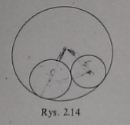
\includegraphics[width=0.4\linewidth]{rys214.png}
\end{figure}

Dwa okręgi styczne zewnętrznie są równocześnie styczne wewnętrznie do trzeciego okręgu o promieniu 3 cm, tak jak na rysunku. Oblicz obwód trójkąta, którego wierzchołkami są środki tych okręgów.

\end{zad}


\begin{proof}
Zadanie na pierwszy rzut oka wygląda na niewykonalne ze względu na zbyt małą ilość danych. Jednak, spójrzmy na informacje którymi dysponujemy:

\begin{enumerate}
\item Duży okrąg ma promień $r = 3$ cm.
\item Pierwszy mały okrąg ma promień $a$.
\item Drugi mały okrąg ma promień $b$.
\item Obwód trójkąta wynosi:
$$a+b + (r-a) + r-b = 2r$$
\end{enumerate}
...co kończy dowód.
\end{proof}

\subsection{Trójkąty i okręgi}

\begin{figure}[H]
\centering
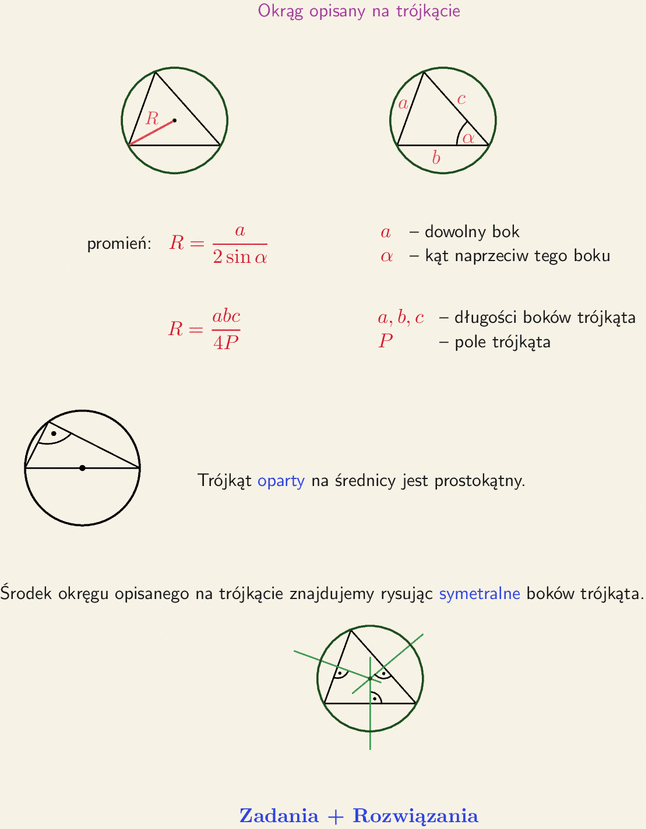
\includegraphics[width=0.8\linewidth]{circle1.png}
\end{figure}

\begin{figure}[H]
\centering
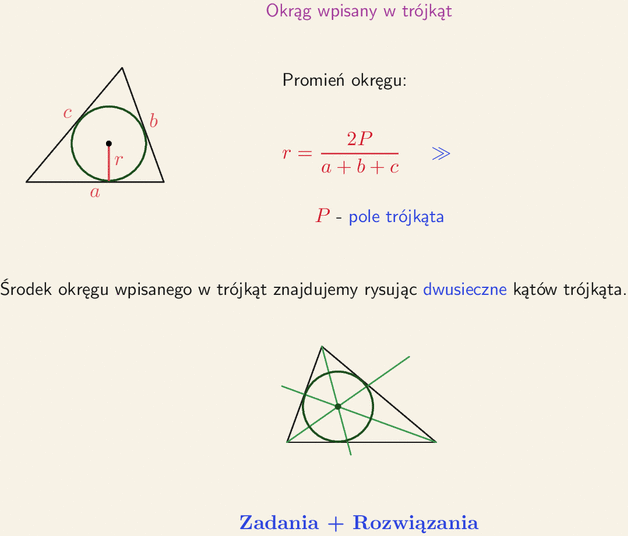
\includegraphics[width=0.8\linewidth]{circle2.png}
\end{figure}

\begin{zad}
W trójkącie ABC bok $|AB| = 8$ cm, bok $|AC| = 10$ cm, a bok $|BC| = 12$ cm. Z punktu O (środka boku BC) zakreślono promieniem OB okrąg przecinający bok AB w punkcie D i bok AC w punkcie E. Oblicz długość odcinków DB i EC.
\end{zad}

\begin{proof}
\begin{figure}[H]
\centering
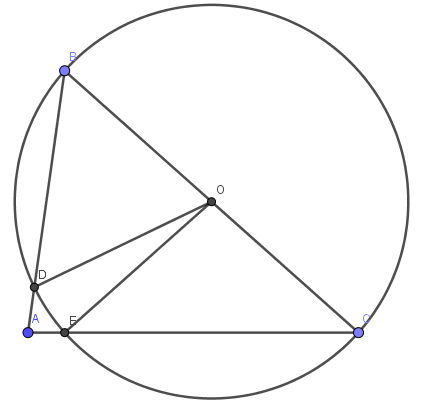
\includegraphics[width=0.5\linewidth]{circle_triangle.png}
\end{figure}
\end{proof}

\begin{zad}
Suma długości boków AC i BC trójkąta ABC wynosi 20 cm. Miary kątów A i B są równe odpowiednio $30^\circ$ i $45^\circ$. Oblicz długości boków AC i BC.
\end{zad}

\begin{zad}
W trójkącie prostokątnym na dłuższej przyprostokątnej jako na średnicy opisano półokrąg. Wyznacz długości półokręgu, jeżeli krótsza przyprostokątna ma długość 30 cm, cięciwa łącząca wierzchołek kąta prostego z punktem przecięcia przeciwprostokątnej z półokręgiem ma długość 24 cm.
\end{zad}

\begin{zad}
Długości boków trójkąta wynoszą 10 cm, 10 cm, 12 cm. Oblicz odległości środka okręgu wpisanego w ten trójkąt od każdego wierzchołka trójkąta.
\end{zad}

\begin{zad}
Dane są dwa koła o promieniach długości 6 dm i 8 dm. Jaką długość ma promień koła, którego pole równa się sumie pól danych kół?
\end{zad}

\begin{zad}
W trójkącie prostokątnym przyprostokątne mają długości: 15 cm i 20 cm. Na krótszej przyprostokątnej jako na średnicy zbudowano okrąg. Oblicz długości odcinków na jakie ten okrąg podzielił przeciwprostokątną.
\end{zad}

\begin{zad}
Oblicz wymiary równoległoboku ABCD, którego obwód wynosi 48 cm. $\frac{|BE|}{|BF|} = \frac57$.

\begin{figure}[h]
\centering
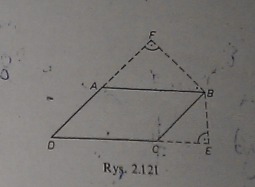
\includegraphics[width=0.4\linewidth]{rys2121.png}
\end{figure}
\end{zad}


\begin{zad}
W trójkącie ABC, w którym miara kąta $C=90^\circ$, długość boku $|AC|=6$ cm, $|BC| = 10$ cm, obrano na boku BC punkt D tak, że miara kąta ADC równa się mierze kąta CAB. Oblicz długości CD i BD.
\end{zad}

\begin{zad}
W trójkącie ABC, którego obwód wynosi 50 cm i $|AC| = |BC|$, poprowadzono środkowe AD i BE. Obwód trójkąta ABE jest o 8 cm większy od obwodu trójkąta ACD. Oblicz długość boków trójkąta ABC.
\end{zad}

\begin{zad}
W trójkąt prostokątny wpisano półokrąg tak, że jego średnica zawarta jest w przeciwprostokątnej i środek tego półokręgu dzieli przeciwprostokątną na odcinki o długościach 15 cm i 20 cm. Oblicz długość łuku zawartego między punktami styczności półokręgu z przyprostokątnymi.
\end{zad}

\section{Bukiety matematyczne}

\subsection{Liczby niewymierne}

\textbf{Liczbą wymierną} nazwiemy każdą liczbę dającą się zapisać w postaci $\frac ab$, gdzie $a, b\in\mathbb Z$ (\footnote{$a, b$ należą do liczb całkowitych - w szkole często miesza się oznaczenie $\mathbb Z$ z $\mathbb C$, które oznacza liczby zespolone. Tutaj będziemy trzymali się notacji akademickiej.}). Każdą liczbę nie dającą się zapisać w postaci ułamka $\frac ab$ wrzucimy zatem w zbiór liczb \textbf{niewymiernych}.

Dowód niewymierności $\sqrt2$: załóżmy, że $\sqrt2$ jest równe $\frac ab$, spróbujemy znaleźć ich wartości. Mamy cztery możliwości:

\begin{enumerate}
\item $a$ oraz $b$ są nieparzyste,
\item $a$ jest parzyste, $b$ jest nieparzyste,
\item $a$ jest nieparzyste, $b$ jest parzyste,
\item $a$ oraz $b$ są parzyste - w tym wypadku redukujemy przypadek do jednego z trzech poprzednich.
\end{enumerate}

Załóżmy że $a$ oraz $b$ są nieparzyste. Wtedy $a^2 = 2b^2$ (po podniesieniu równania $\sqrt 2 = \frac ab$ do kwadratu), co jednak prowadzi do sprzeczności, bowiem kwadrat liczby nieparzystej jest parzysty. Usuwamy pierwszą możliwość.

Załóżmy zatem że $a$ jest parzyste a $b$ jest nieparzyste. $a$ możemy przedstawić jako $2\cdot x$. Po podniesieniu do kwadratu mamy $4x^2 = 2b^2$, co redukuje się do $2x^2=b^2$. Ponownie, założyliśmy nieparzystość $b$, więc przypadek jest sprzeczny.

Ostatnia możliwość: $a$ jest nieparzyste, $b$ jest parzyste. Po podniesieniu do kwadratu równania $\sqrt 2 = \frac{a}{2x}$ dostajemy $a^2 = 8x^2$... ale $a$ miało być nieparzyste. Znowu sprzeczność.

Przypadek czwarty możemy zredukować do jednego z trzech pozostałych, zatem nie ma co rozważać go osobno.

\textbf{Zadanie dodatkowe:} Spróbuj udowodnić w analogiczny sposób niewymierność liczby $\sqrt3$.

\subsection{Ułamki łańcuchowe}

Istnieje pewien intrygujący sposób przedstawiania liczb, nazywany \textbf{ułamkiem łańcuchowym}:

$$ x = a + \frac{1}{b+\frac{1}{c+\frac1{d+...}}}$$

Dla każdej liczby wymiernej istnieje skończona reprezentacja tej postaci (czynniki $a,b,c,d$ są naturalne). Co interesujące, liczby niewymierne również można przedstawiać w tej formie - będzie ona jednak nieskończona. Każdy ułamek łańcuchowy postaci nieskończonej będzie liczbą niewymierną.\footnote{Dowód możemy przeprowadzić pokazując, że liczba kroków dla liczby wymiernej $\frac{a}{b}$ musi być skończona. Dlatego każda liczba o nieskończonej liczbie kroków nie będzie miała postaci $\frac ab$.}

\begin{zad}
Oblicz wartość wyrażenia:

$$x = 1+\frac1{1+\frac1{1+1}}$$
\end{zad}

\begin{zad}
Znajdź liczby naturalne $a,b,c,d$ spełniające równanie:

$$\frac{151}{115}=a+\frac1{b+\frac1{c+\frac1d}}$$
\end{zad}
\begin{zad}
Znajdź postać w reprezentacji ułamka łańcuchowego dla liczby $\frac{225}{157}$.
\end{zad}

\begin{zad}
Znajdź reprezentację ułamka łańcuchowego dla $\sqrt{2}$.

\textbf{Podpowiedź}: $\sqrt{2} = 1 + (\sqrt{2}-1) = 1+\frac1{1+\sqrt{2}}$.
\end{zad}
\newpage
\section{Geometria}

Na początek małe zadanie z trygonometrii:

\begin{zad}
Dane są długości dwóch przyległych boków trójkąta oraz kąt między nimi:

\begin{figure}[h]
\centering
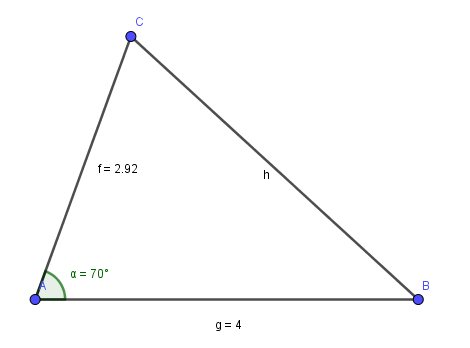
\includegraphics[width=0.5\linewidth]{triangle.png}
\end{figure}
Oblicz pole trójkąta oraz długość trzeciego boku.
\end{zad}

\begin{zad}
W trójkącie równobocznym geometryczny środek (będący równocześnie środkiem okręgu opisanego na trójkącie) dzieli wysokość na dwa odcinki. Udowodnij, że proporcja między tymi odcinkami jest równa $1:2$.
\end{zad}

\begin{zad}[Twierdzenie o kącie wpisanym] Udowodnij, że relacja pomiędzy kątami $CBA$ oraz $CDB$ ma się jak $2:1$.
\begin{figure}[h]
\centering
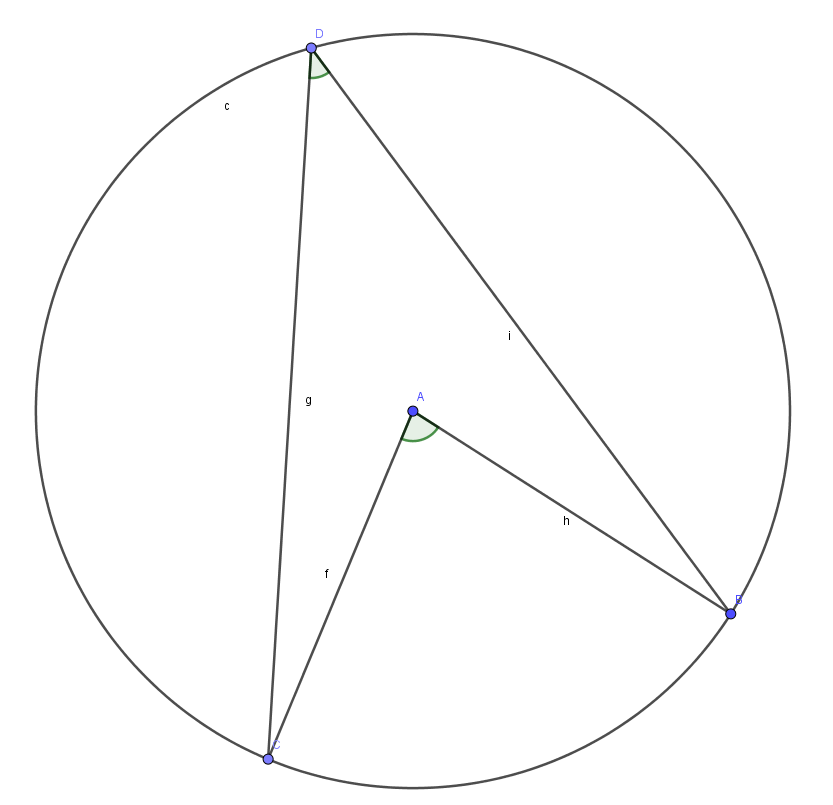
\includegraphics[width=0.5\linewidth]{circle.png}
\end{figure}
\end{zad}

\section{Liga zadaniowa}

\subsection{Równania z wartością bezwzględną}



\section{Teoria funkcji}

Funkcją nazwiemy operację matematyczną przypisującą danej wartości wejściowej wartość wyjściową zgodnie z określoną regułą. I tyle! Tak prosta definicja pozwala na nałożenie całkiem dobrych ram na naszą teorię.

Po pierwsze - niemożliwe jest, aby funkcja dla konkretnej wartości wejściowej (\textbf{argumentu}) zwracała różne wartości wyjściowe (\textbf{wartości funkcji}, albo po prostu: \textbf{wartości}).


\end{document}
